\chapter{Versuchsdurchführung}

\section{Versuchsaufgabe 1: Statische Messung der Diodenkennlinie}

Folgende Dioden werden untersucht:

\begin{itemize}
    \item{D1:} Silizium-Diode MRA4004, max. Sperrspannung $400 \si{\volt}$; max. Durchlassstrom $1000 \si{\milli\ampere}$;
    \item{D2:} Schottky-Diode 10BQ015, max. Sperrspannung $15 \si{\volt}$; max. Durchlassstrom $1000 \si{\milli\ampere}$.
\end{itemize}

Zur statischen Messung der Diodenkennlinie ($I = f(U)$) wird die Diode in Reihe mit einem Widerstand $R = 100 \si{\ohm}$ geschaltet.
In Durchlassrichtung der Dioden wird spannungsrichtig gemessen (siehe Voraufgabe F):
Die Spannung $U$ wird dabei nur über die Diode mit dem analogen Messgerät (UNIGOR 4P) gemessen, 
der Strom $I$ hingegen mit dem digitalen Multimeter (DMM), aufgrund dessen schlechteren Genauigkeit.

In Sperrrichtung wird umgekehrt verfahren: Für die stromrichtige Messung wird die Spannung $U$ über Diode und analogem Amperemeter gemessen,
der Strom $I$ hingegen mit dem DMM.

% Schaltungsskizze?

Aus unserer Messung bei geeigneten ausgewählten Spannungswerten ergeben sich folgende Kennlinien:
% Plots
% Auswertung


\section{Versuchsaufgabe 2: Oszillogramm der Diodenkennlinie}
\label{sec:A2}

Nun soll die Kennlinie der Diode mit einem Oszilloskop aufgenommen werden.
Dies wird umgesetzt, indem eine Wechselspannung an die Diode angelegt wird, 
die dann in Durchlassrichtung und Sperrrichtung abwechselnd wirkt.
Um den Strom, der durch die Diode fließt, zu messen, wird mithilfe der Black Box die Spannung vor und nach dem Widerstand $R = 100 \si{\ohm}$
zu einem Referenzpotential gemessen (siehe \ref{fig:2_strom}).

\begin{figure}[H]
    \centering
    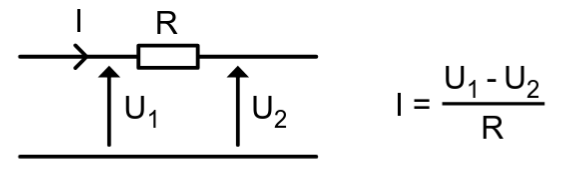
\includegraphics[width=0.5\textwidth]{figs/2/strom.png}
    \caption{Zur Strommessung}
    \label{fig:2_strom}
\end{figure}

Dadurch erhält man als Ausgang eine Spannung, die proportional zum Strom $I$ ist, der durch die Diode fließt.
Betrachtet man nun diese Spannung und die Eingangswechselspannung am Oszilloskop im XY-Modus, und steigert die Amplitude der Wechselspannung,
so erscheint die Kennlinie der Diode als Oszillogramm.

% Schaltungsskizze?

Zusätzlich zu den Dioden D1 und D2 wird jetzt auch eine Zener-Diode ZD untersucht.
Es ergeben sich folgende Kennlinien:

\begin{figure}[H]
    \centering
    \begin{subfigure}[b]{0.45\textwidth}
        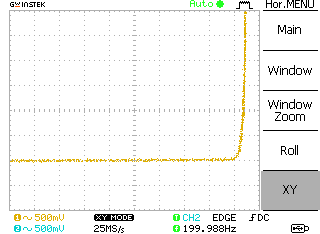
\includegraphics[width=\textwidth]{figs/2/DS0000.png}
        \caption{D1}
        \label{fig:2_D1}
    \end{subfigure}
    \hfill
    \begin{subfigure}[b]{0.45\textwidth}
        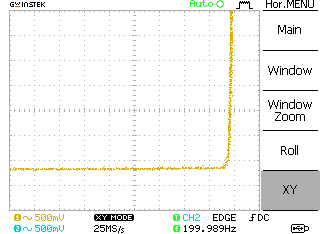
\includegraphics[width=\textwidth]{figs/2/DS0001.png}
        \caption{D2}
        \label{fig:2_D2}
    \end{subfigure}
    \vspace{0.5em}
    \begin{subfigure}[b]{0.45\textwidth}
        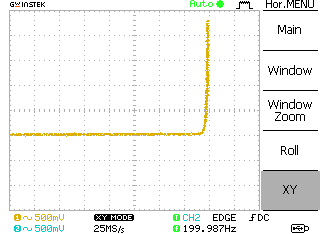
\includegraphics[width=\textwidth]{figs/2/DS0002.png}
        \caption{ZD}
        \label{fig:2_ZD_1}
    \end{subfigure}
    \hfill
    \begin{subfigure}[b]{0.45\textwidth}
        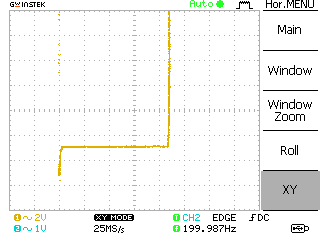
\includegraphics[width=\textwidth]{figs/2/DS0003.png}
        \caption{ZD in größerem Bereich}
        \label{fig:2_ZD_2}
    \end{subfigure}
    \caption{Oszillogramme der Diodenkennlinien}
\end{figure}


Die charakteristischen Kennlinien der Dioden sind zu erkennen. 
Man erkennt, dass die Schottky-Diode D2 eine leicht geringere Durchlassspannung (ca. $\SI{1,8}{\volt}$) aufweist als die Silizium-Diode D1 (ca. $\SI{2,0}{\volt}$).
Die der Zener-Diode ZD ist mit ca. $\SI{1,3}{\volt}$ noch einmal deutlich geringer.
Es fällt auf, dass diese Werte nicht nah am erwarteten Wert von $\SI{0,6}{\volt}$ liegen.
Außerdem fällt auf, dass die Kennlinien in den konstanten Bereichen nicht auf 0 sind, 
obwohl wir mit einer sehr niedrigen Wechselspannung von ca. $\SI{20}{\milli\volt}$ verifiziert hatten, dass der Nullpunkt im Ursprung des Oszilloskops liegt.
Während unserer Aufzeichnung konnten wir verstellen, dass durch die kontinuierliche Änderung der Spannung die Kennlinie sich nach unten und rechts (??) verschiebt,
also sowohl in $x$- als auch in $y$-Richtung.
Dies erklärt auch die Abweichung der Durchlassspannung von den erwarteten Werten.
Dieses Phänomen konnten wir auch bei anderen Komilitonen unserer Gruppe beobachten. 
Es scheint also ein generelles Problem zu sein, das nicht nur auf unsere Messung zurückzuführen ist.
Die Ursache hierfür ist uns nicht bekannt.
% AI AM KOCHEN
% , aber es könnte an der Black Box liegen, die wir für die Messung verwendet haben.
% Die Black Box könnte eine gewisse Eigenkapazität besitzen, die die Spannung beeinflusst, die wir messen.
% Eine weitere Möglichkeit wäre, dass die Black Box nicht für Wechselspannungen geeignet ist, 
% sondern nur für Gleichspannungen, und die Messung daher nicht korrekt ist.

Als Zenerspannung erhalten wir einen abgelesenen Wert von $(2,9 \pm 0,1)\si{\volt}$ (Unsicherheit abgeschätzt).


\section{Versuchsaufgabe 3: Oszillogramm des Einweggleichrichters}

Aus dem unteren Teil des Dioden-Schaltbretts wird ein Einweggleichrichter aufgebaut (siehe \ref{fig:3_gleichrichter}a).

\begin{figure}[H]
    \centering
    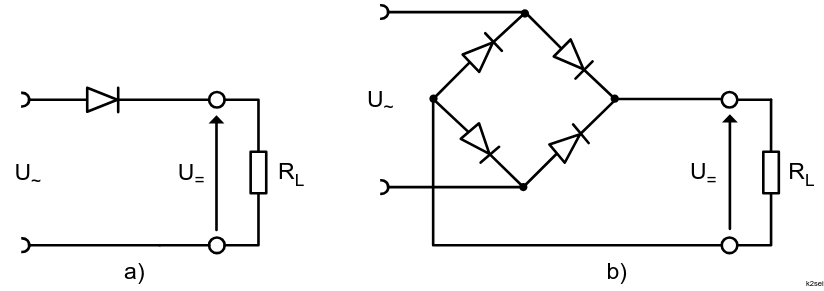
\includegraphics[width=0.5\textwidth]{figs/3/gleichrichter.png}
    \caption{Ein- und Zweiweggleichrichter}
    \label{fig:3_gleichrichter}
\end{figure}

Die gleichzurichtende Wechselspannung von \SI{15}{\volt} wird einem separaten massefreien Netzgerät entnommen (kleiner grauer Kasten). 
Das Potentiometer auf dem Schaltbrett als variable Last für die gleichgerichtete Spannung wird auf den maximalen Wert von \SI{8}{\kilo\ohm} eingestellt.
Es werden zusätzlich verschiedene Kondensatoren parallel zur Last hinzugeschaltet.
Die Spannung $U$ über der Last wird mitsamt der mittleren Höhe der Gleichspannung $U_{avg}$ und der Brumm-Amplitude $U_{pp}$ am Oszillographen angezeigt:

\begin{figure}[H]
    \centering
    \begin{subfigure}[b]{0.45\textwidth}
        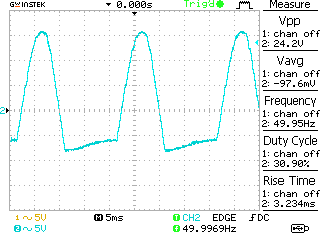
\includegraphics[width=\textwidth]{figs/3/DS0009.png}
        \caption{ohne Kondensator}
        \label{fig:3_C0}
    \end{subfigure}
    \hfill
    \begin{subfigure}[b]{0.45\textwidth}
        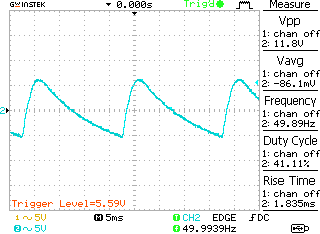
\includegraphics[width=\textwidth]{figs/3/DS0010.png}
        \caption{$C=\SI{2,2}{\micro\farad}$}
        \label{fig:3_C1}
    \end{subfigure}
    \vspace{0.5em}
    \begin{subfigure}[b]{0.45\textwidth}
        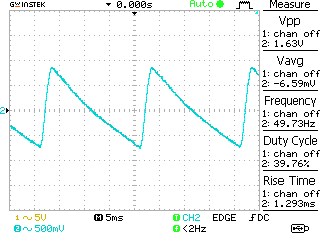
\includegraphics[width=\textwidth]{figs/3/DS0011.png}
        \caption{$C=\SI{22}{\micro\farad}$}
        \label{fig:3_C2}
    \end{subfigure}
    \hfill
    \begin{subfigure}[b]{0.45\textwidth}
        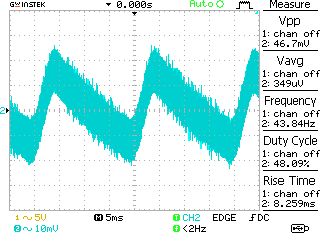
\includegraphics[width=\textwidth]{figs/3/DS0012.png}
        \caption{$C=\SI{1000}{\micro\farad}$}
        \label{fig:3_C3}
    \end{subfigure}
    \caption{Oszillogramme und Werte des Einweggleichrichters}
\end{figure}

Es ist wieder zu erkennen, dass die Spannungskurve in $y$-Richtung verschoben ist (siehe \ref{sec:A2}).
Die Bereiche, in denen die Spannung 0 sein sollte, liegen im negativen Bereich.
Das kann nicht richtig sein, da der Gleichrichter genau das verhindern sollte.
Dadurch sind die gemessenen Werte für $U_{avg}$ unbrauchbar.
Dennoch entspricht der zeitliche Verlauf der Kurve den Erwartungen, und auch die Brumm-Amplitude $U_{pp}$ sollte davon unbeeinflusst sein.
Im Folgenden werden wir also nur diese Aspekte betrachten können.

Ohne Kondensator (\ref{fig:3_C0}) stimmt das Oszillogramm gut mit der erwarteten Form (siehe \ref{fig:VA_D_a}) überein, 
der positive Teil der Sinusspannung ist gut zu erkennen.
Mit steigender angeschlossener Kapazität $C$ wird die Maximalspannung immer kleiner (auch erkennbar an den kleiner werdenden Beträgen der Werte $U_{avg}$), 
und dementsprechend auch die Brumm-Amplitude $U_{pp}$.
Zudem wird der Abfall der Spannung in jedem Zyklus langsamer.
Diese beiden Resultate sind genau die Ergebnisse der Glättung durch den Kondensator.
Auffällig ist außerdem auch, dass bei $C=\SI{1000}{\micro\farad}$ (\ref{fig:3_C3}) die Spannung im Vergleich zu den anderen Fällen nur noch sehr klein ist.
Das liegt daran, dass der Großteil der Eingangsspannung über den großen Kondensator abfällt (der Kondensator wird geladen), und nur ein sehr kleiner Teil über die Last.
Das Ergebnis davon ist dadurch eine Spannung, die zwar sehr geglättet ist, aber auch nur noch eine sehr kleine Amplitude hat.


\section{Versuchsaufgabe 4: Oszillogramm des Zweiweggleichrichters}

Aus dem oberen Teil des Dioden-Schaltbretts wird nun ein Zweiweggleichrichter aufgebaut (siehe \ref{fig:3_gleichrichter}b).
Der Aufbau und die Messungen erfolgen ansonsten analog zu Versuchsaufgabe 3.

\begin{figure}[H]
    \centering
    \begin{subfigure}[b]{0.45\textwidth}
        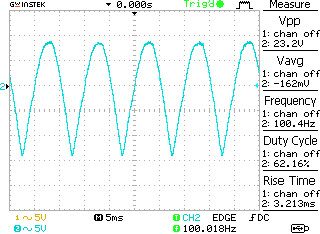
\includegraphics[width=\textwidth]{figs/4/DS0000.png}
        \caption{ohne Kondensator}
        \label{fig:4_C0}
    \end{subfigure}
    \hfill
    \begin{subfigure}[b]{0.45\textwidth}
        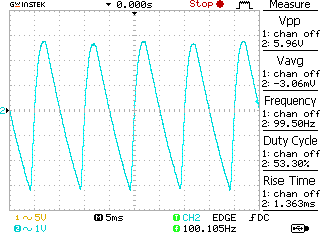
\includegraphics[width=\textwidth]{figs/4/DS0001.png}
        \caption{$C=\SI{2,2}{\micro\farad}$}
        \label{fig:4_C1}
    \end{subfigure}
    \vspace{0.5em}
    \begin{subfigure}[b]{0.45\textwidth}
        \centering
        fehlt
        \caption{$C=\SI{22}{\micro\farad}$}
        \label{fig:4_C2}
    \end{subfigure}
    \hfill
    \begin{subfigure}[b]{0.45\textwidth}
        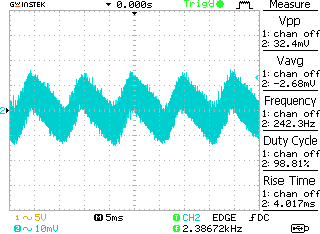
\includegraphics[width=\textwidth]{figs/4/DS0002.png}
        \caption{$C=\SI{1000}{\micro\farad}$}
        \label{fig:4_C3}
    \end{subfigure}
    \caption{Oszillogramme und Werte des Zweiweggleichrichters}
\end{figure}


Wir haben leider vergessen, ein Oszillogramm für $C=\SI{22}{\micro\farad}$ aufzunehmen.

Es ist wieder die Verschiebung in $y$-Richtung zu erkennen (siehe \ref{sec:A2}).
Die daraus resultierenden Probleme bleiben also wie bei Versuchsaufgabe 3 bestehen.

Die Form der Kurven ohne Kondensator entspricht wieder gut dem erwarteten Bild (siehe \ref{fig:VA_D_b}).
Die Auswertung kann 1:1 von Versuchsaufgabe 3 übernommen werden, da alle Beobachtungen analog sind.